% Utilize o comando \section para criar uma seção
% Utilize o comando \subsection para criar subseção

%Fundamentação teórica 
\chapter{FUNDAMENTAÇÃO TEÓRICA}
\label{chap:fundamentacao}

Neste capítulo serão apresentadas as bases teóricas do trabalho, fundamentando o conhecimento necessário para a criação da assistente virtual. O capítulo abordará conceitos da conversação natural e dos comandos que serão passados para o sistema, bem como as tecnologias e ferramentas de \textit{Hardware}, \textit{Softwares} e comunicação necessária para o funcionamento do fluxo de automação deste. Além disso, também será abordado os conceitos abstratos do que são assistentes virtuais de voz, e como é dado o conhecimento e entendimento da linguagem humana de uma perspectiva científica, tendo como objetivo introduzir no leitor o entendimento destes sistemas e embasar a importância de seu uso.

%cntrl + T comentar varias linhas e ctrl U descomentar

\section{Assistentes virtuais de voz}

	Assistentes virtuais de voz são sistemas computacionais que servem para auxilio e automatização de tarefas humanas, realizando por meio de reconhecimento de linguagem natural tarefas diversas, sejam elas profissionais, sociais, ou domésticas. Esses sistemas combinam técnicas de Inteligência Artificial, Processamento de Linguagem Natural (PLN) e Reconhecimento de Fala para interpretar intenções humanas, gerar respostas e comandos adequados \cite{russell2021}. O assistente faz o papel de um agente inteligente, como citado também por Russel e Norvig. O fluxo de interação entre Agente e Ambiente é mostrado na \autoref{fig:fluxo_ambi_agente}. 

\begin{figure}[!ht]
\centering
\caption{Fluxo de interação Agente - Ambiente.}
\label{fig:fluxo_ambi_agente}   
  \centering
  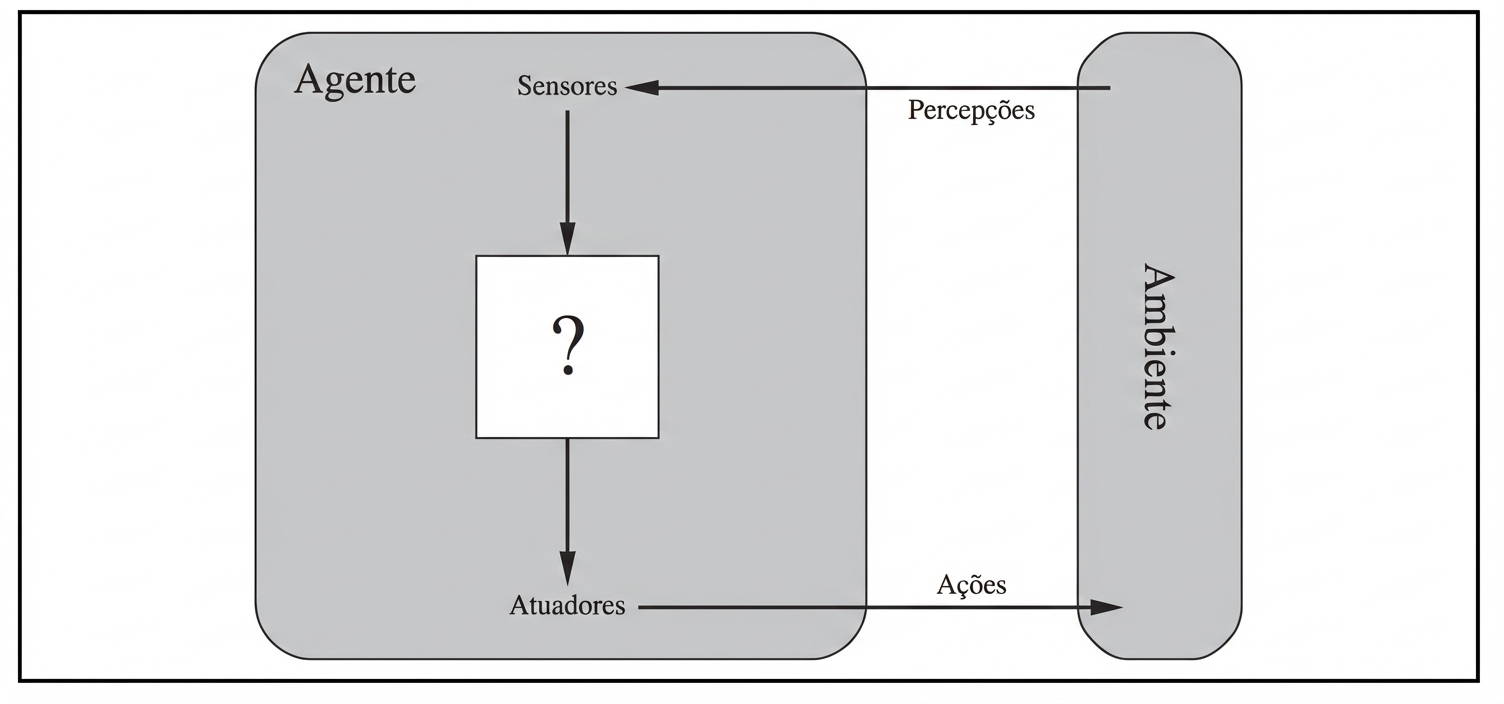
\includegraphics[width=100mm]{Imagem/CAP2/fluxo_ambi_agente.png}\\[0.10cm]
Fonte: Adaptado de (\cite{russell2021}, cap. 2).
\end{figure}

Como cita Marcela Pedroso em \cite{maues2019dissertacao}, os assistentes virtuais de voz tem a voz e o texto como principal fonte de entrada de dados (\textit{inputs}), que podem ser obtidas do assistente em forma de texto digitado pelo usuário, em formato de conversa (\textit{chat}), ou em forma de fala do usuário, como utilizado em sistemas citados anteriormente (\textit{Siri, Alexa, Google Assitant}). Os assistentes também podem adotar formas de lidar com determinado usuário, como voz, opinião e até humor, o que serve para tornar o sistema ainda mais amigável ao ser humano.


\section{Modelo de Linguagem em Grande Escala (LLMs)}
Modelos de Linguagem em Grande escala, também conhecidos como \textit{Large Language Models (LLMs)} são modelos de  baseados em redes neurais profundas (\textit{Deep Learning}), treinados com uma vasta quantidade de palavras e dados, sendo capazes de aprender padrões e preverem suas próximas reações baseado em estatística o que os tornam focados em linguagem natural e capazes de adaptar-se ao usuário \cite{ibm_llm}. Os LLMs também são treináveis e possuem parâmetros configuráveis, e quando bem estruturados podem ser focados em uma tarefa específica, como automação residencial, por exemplo. No trabalho "Desafios e aplicações de Modelos de Linguagem em Grande Escala"\cite{kaddour2023llm}, o autor explica como é dado a construção de um LLM e explica alguns desafios sobre os modelos, bem como usos típicos, incluindo o de conversação.

Como cita Julian Varas et al. \cite{varas2023llm}, os LLMs ganharam alta notoriedade nos últimos anos por sua capacidade de gerar texto em linguagem natural como saída, possibilitando sua utilização para diversas tarefas como criação de roteiros, pesquisa e até conversação, visto que os modelos atuais são capazes de entender contexto e situação do seu usuário.



\subsection{O modelo TinyLlama}
O TinyLlama é uma modelo de linguagem compacto em código aberto com aproximadamente 1,1 a 2 bilhões de parâmetros (que são os pesos que determinam como o modelo aprende durante seu treinamento) e cerca de 3 trilhões de tokens , que são pequenas palavras que os modelos usam para processar e gerar linguagem, contexto e raciocínio \cite{Nvidia_tokens}, baseado na arquitetura Llama 2, e foi criado para ser embarcado em dispositivos com poucos recursos computacionais, como notebooks, celulares e até mesmo em sistemas embarcados como a \textit{Raspberry Pi} \cite{tinyllama2023}. Sua arquitetura simples faz com que o modelo se torne leve, com aproximadamente 500MB, e capaz de ser funcional e fluído em dispositivos com Memória Memória de Acesso Aleatório (RAM) de 2 GB ou superior. 

\section{Raspberry PI}
A Raspberry PI (Rasp) é um microcomputador de placa única compacto de baixo custo, utilizado para fins educacionais, acadêmicos e industriais \cite{raspberrypi_ifrn}. Desenvolvida pela Raspberry Pi Fundation em 2011, a placa possibilita o uso de periféricos, que a depender da versão podem contemplar Entrada HDMI (\textit{High-Definition Multimedia Interface}), Entradas USB (\textit{Universal Serial Bus}) para Mouse e Teclado, Conector Ethernet RJ45, Cartão SD (\textit{Secure Digital}), o que possibilita seu uso como um computador pessoal (PC - \textit{Personal Computer}) e faz com que a Rasp se "encaixe perfeitamente como um dispositivo servidor que trabalha na rede com dispositivos clientes" (trecho traduzido de \cite{VUJOVIC2015153}).

\begin{figure}[H]
	\centering
	\caption{Rasp funcionando como um PC.}
	\label{fig:rasp_pc}   
	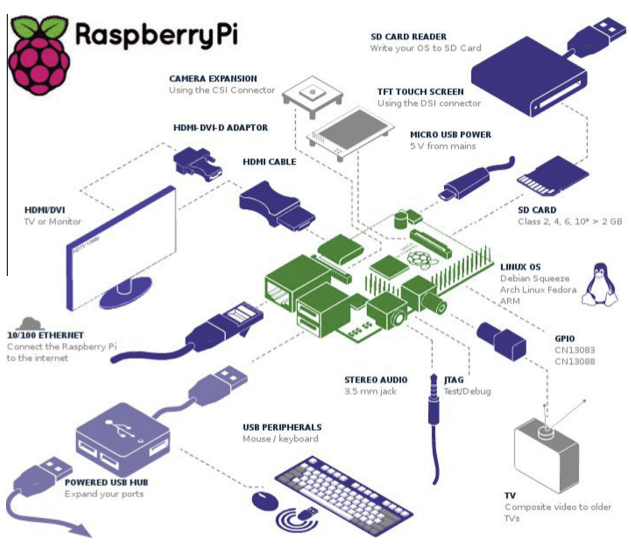
\includegraphics[width=0.9\textwidth]{Imagem/CAP2/rasp_perifericos.png}\\[0.11cm]
	Fonte: \cite{VUJOVIC2015153}.
\end{figure}

Além das diversas posibilidades de periféricos, a Rasp conta com várias possibilidades de sistemas operacionais a serem instalados, como o \textit{Ubuntu}, \textit{Chromium OS}, \textit{Windows 10 IoT}, dentre outros (\cite{OS_rasp}), porém, o que se destaca é o seu sistema operacional customizado feito para a Rasp, o \textit{Raspbian}, que deriva do \textit{Debian Linux} e possui boa estabilidade e alta compatibilidade, além de uma perfomance boa mesmo em hardwares com baixo poder computacional, além de ser uma Ferramenta de Código Aberto (\textit{Open Source}) \cite{RaspUserGuide}. 

\subsection{O modelo PI 4B}
A Rasperry Pi  possui diversos modelos, cada um com suas diferenças de custo, poder computacional (Mémoria RAM), interfaces e processamento. O seu modelo de quarta geração (\textit{Raspberry 4 Model B}) trabalha com um processador de arquitetura ARM de quatro núcleos, o Broadcom BCM2711 \cite{raspberrypi_foundation}. Esta versão também conta com Bluetooth 5.0 e Wi-fi, permitindo ser integrada a redes de comunicação com e sem fio (\textit{Wired e Wireless}) através da utilização de seus mais diversos protocolos, como por exemplo o de Transporte de Telemetria de Enfileiramento de Mensagens (MQTT) . Para o modelo 4B são disponibilizadas opções com 2GB, 4GB, e 8GB de memória RAM.

\begin{figure}[!ht]
	\centering
	\caption{Raspberry Pi 4 Model B.}
	\label{fig:4-model-b}   
	\centering
	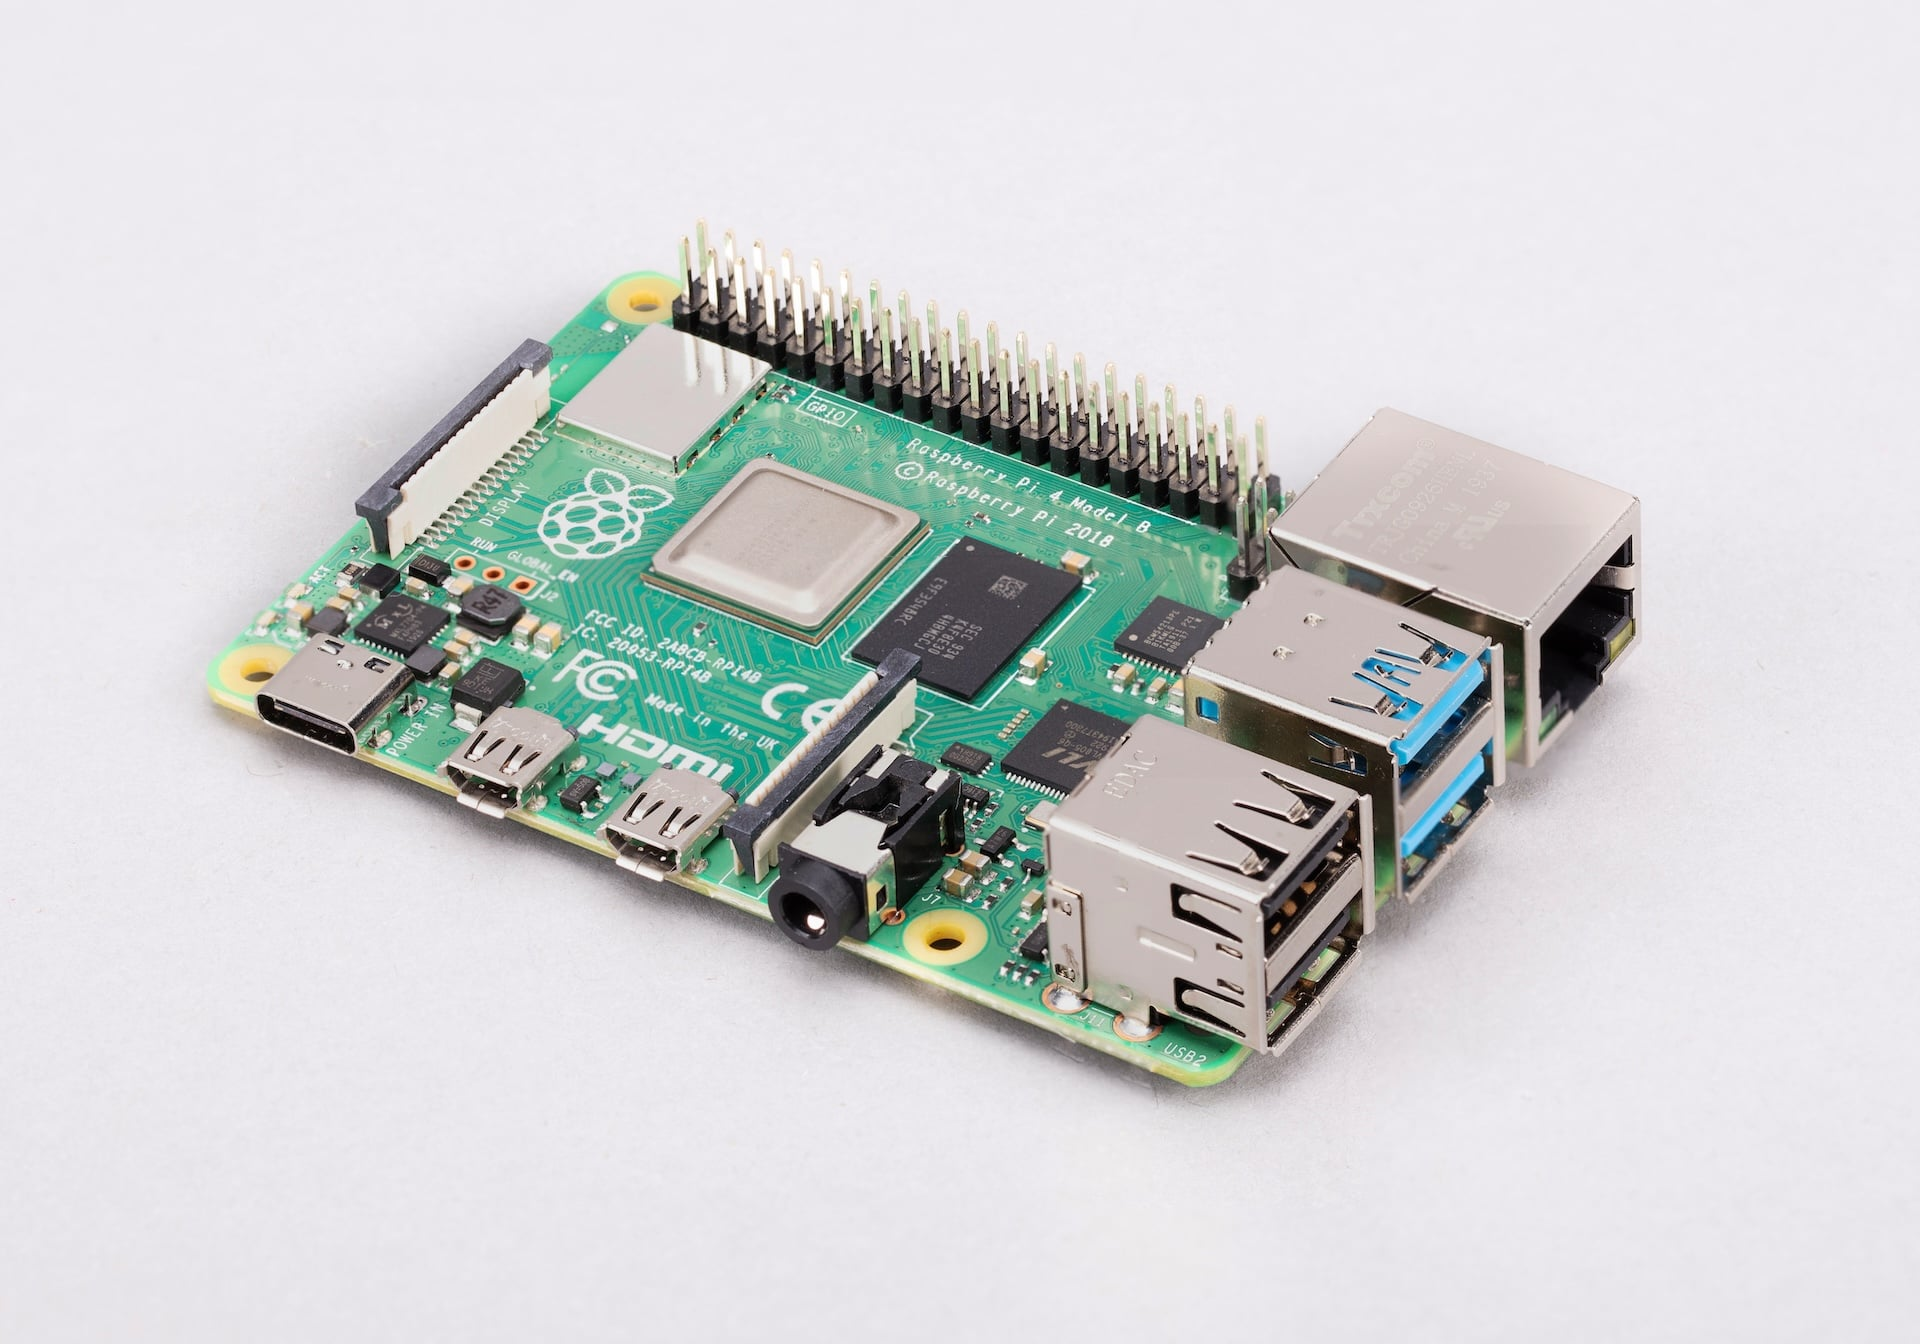
\includegraphics[width=100mm]{Imagem/CAP2/4-model-b.jpg}\\[0.10cm]
	Fonte: (\textit{Raspeberry Pi Foundation}).
\end{figure}

\subsubsection{Entradas e Saídas do Hardware}
Além disso, a placa integrada possui entradas e saídas digitais e analógicas para utilização de automações diversas dentro do própio Hardware, o modelo 4B possui 40 pinos de \textit{GPIO (General-Purpose Input/Output)}, que são programáveis via linguagem Python ou C dentro do própio sistema operacional do computador utilizando bibliotecas e interfaces já instaladas em seus softwares nativos. A figura a seguir mostra o esquema dos \textit{GPIOS} da Rasp e a função de cada pino na placa.

\begin{figure}[!ht]
	\centering
	
	\caption{Raspberry Pi 4 Model B - Descrição de \textit{GPIOS}.}
	\label{fig:rasp_pi_mapa}   
	\centering
	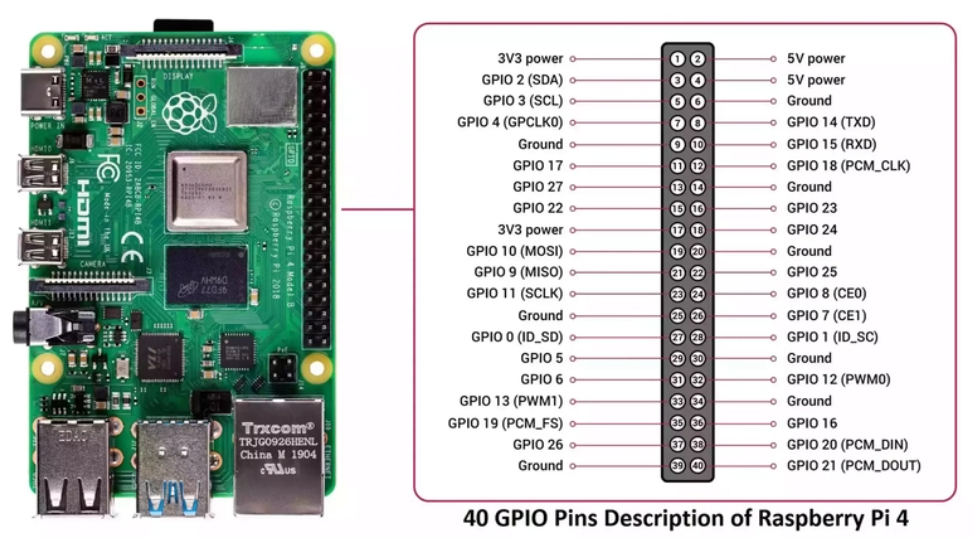
\includegraphics[width=100mm]{Imagem/CAP2/rasp_pi_mapa.png}\\[0.10cm]
	Fonte: \cite{Dev_RaspPi}.
\end{figure}

\section{ESP 8266}
O ESP8266 é um microcontrolador compacto desenvolvido pela empresa \textit{Espressif Systems}. Projetado com um  processador Tensilica de 32-bits, a placa integrada que contém o chip de processamento e circuito integrado chamado \textit{NodeMCU}, é feita para permitir a conexão de equipamentos eletrônicos à internet e dispositivos como atuadores e sensores de forma simples e eficiente, com aplicações diversas em automação residencial, internet das coisas (IoT) e monitoramento remoto \cite{espressif_esp8266}. A \autoref{fig:esp8266_foto} mostra a placa de desenvolvimento NodeMCU ESP8266.

\begin{figure}[H]
	\centering	
	\caption{Placa integrada Node MCU ESP8266.}
	\label{fig:esp8266_foto}   
	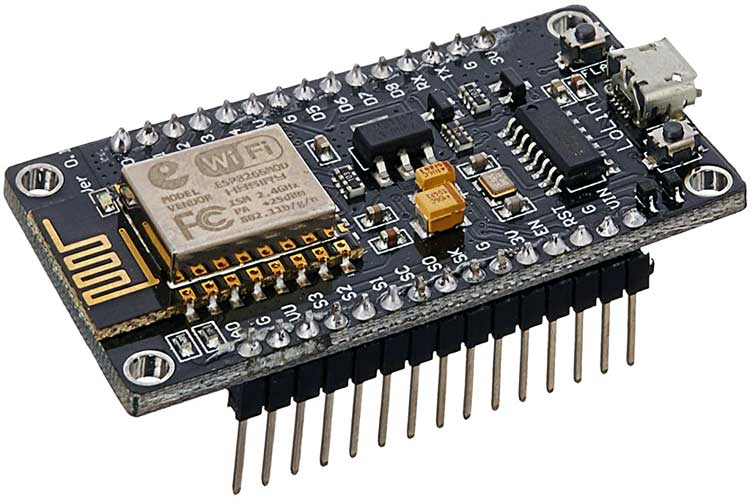
\includegraphics[width=100mm]{Imagem/CAP2/esp_8266.jpg}\\[0.10cm]
	Fonte: (COMPONENTS101, 2026).
\end{figure}

Segundo o manual técnico de referência da ESP8266 fornecido pela Espressif \cite{esp8266_manual}, a placa conta com 17 pinos de \textit{GPIO} que podem ser configurados de acordo com a preferência do usuário, dentre eles estão pinos que podem ser utilizados para outras funções e formas de sinal, como Protocolo serial I2C (\textit{Inter-Integrated Circuit}) e  Modulação de Largura de Pulso PWM (\textit{Pulse-Width Modulation}). Além disso, o microcontrolador conta com \textit{Bluetooth} nativo e \textit{WiFi}, o que possibilita criação de sistemas com interfaces Web e integrações com os diversos protocolos de redes de comunicação, como o de Transporte de Telemetria de Enfileiramento de Mensagens (MQTT). A \autoref{fig:esp8266_pin} detalha os \textit{GPIOS} da placa e suas possibilidades de uso.

\begin{figure}[H]
	\centering	
	\caption{Node MCU ESP8266 - Descrição de \textit{GPIOS}.}
	\label{fig:esp8266_pin}   
	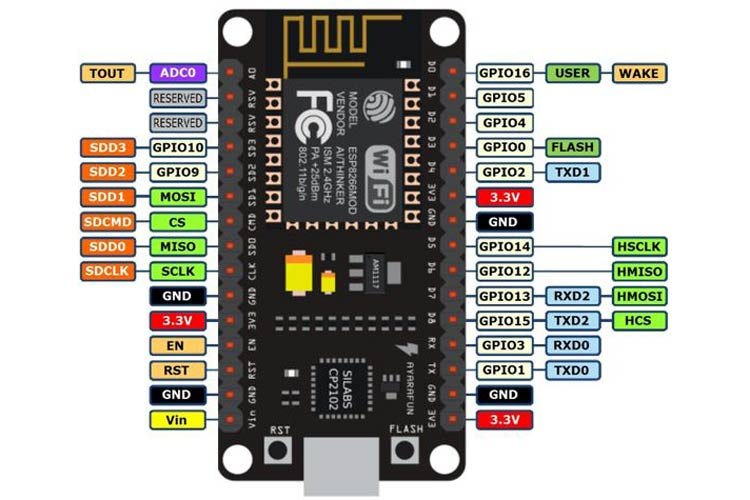
\includegraphics[width=100mm]{Imagem/CAP2/esp_8266_pinout.jpg}\\[0.10cm]
	Fonte: (COMPONENTS101, 2026).
\end{figure}


A programação da ESP8266 pode ser feita pela interface de programação ''Arduino IDE'' utilizando a linguagem C ou C++ e conectando a placa via USB para alimentação e transmissão/recebimento de dados do chip e do circuito integrado \textit{NodeMCU}. A \autoref{fig:arduino_ide_esp} mostra um exemplo de programação para ESP8266 como um código simples para ligar e desligar o pino GPIO 2 a cada 1 segundo utilizando a interface ''Arduino IDE''.

\begin{figure}[H]
	\centering	
	\caption{Exemplo de programação do ESP8266.}
	\label{fig:arduino_ide_esp}   
	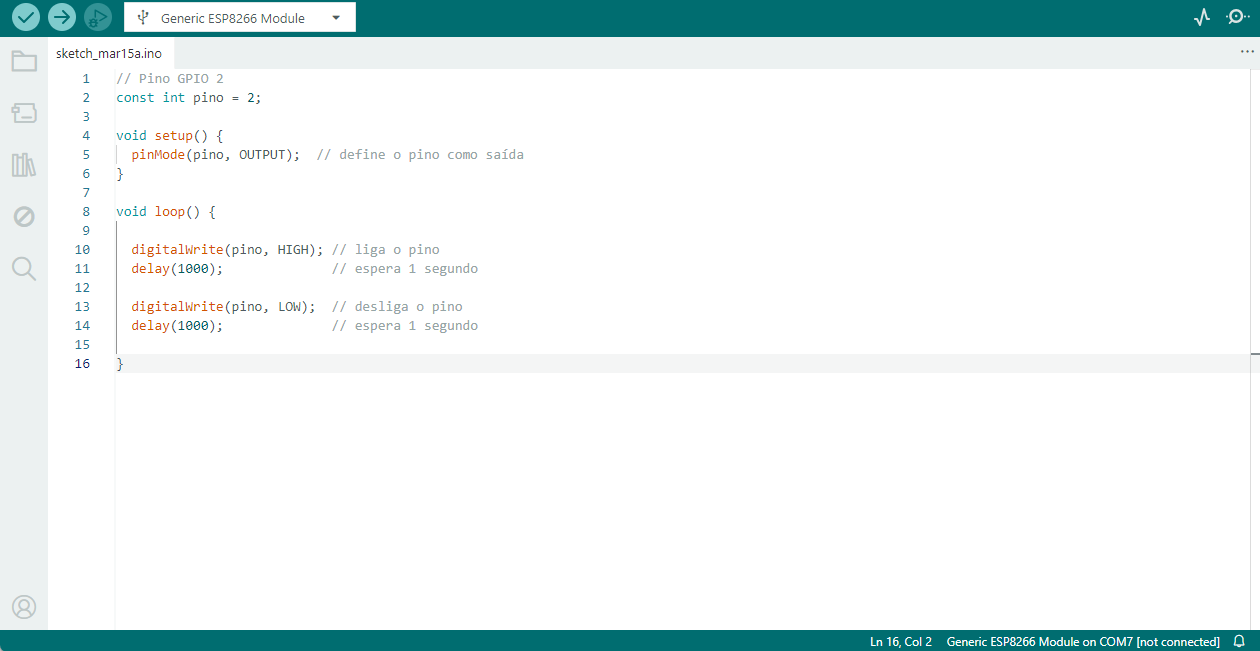
\includegraphics[width=140mm]{Imagem/CAP2/exemplo_arduinoide.png}\\[0.10cm]
	Fonte: (Próprio Autor, 2026).
\end{figure}

\underline{}

\section{O protocolo MQTT}
O protocolo de Transporte de Telemetria de Enfileiramento de Mensagens, ou MQTT (Message Queuing Telemetry Transport), é um protocolo de rede amplamente utilizado em ambientes industriais e residenciais devido a sua flexibilidade, leveza e arquitetura considerada simples. O protocolo foi criado na década de 90 pela IBM e Eurotech para corrigir alguns pontos que o protocolo anterior, o de Transferência de Hipertexto (HTTP) deixa a desejar, e tem a finalidade de fornecer baixo consumo de rede, banda e software, além de funcionamento em redes instáveis. Por estes motivos, o MQTT é muito utilizado em comunicação de Máquina para Máquina (M2M) e conectividade de Internet das Coisas (IoT) \cite{mqtt_site}.


Segundo o guia técnico da versão 5.0, feito pela organização OASIS \cite{mqtt_v5_oasis}, que é atual responsável para padronização do MQTT, o protocolo funciona em modelo Publicador/Assinante (\textit{Publish/Subscribe}). De maneira resumida, um servidor, chamado de \textit{Broker} publica as informações em tópicos e os clientes que desejarem acessá-las assinam este tópico, assim, sempre que o pacote contendo a mensagem final (chamado de \textit{Payload}) for publicado pelo servidor, poderá ser acessado pelo cliente, outra vantagem do MQTT é que o \textit{Payload} pode ser um dado de diversos formatos, como Texto, JSON, binário, dados analógicos de sensores e comandos. Citando uma aplicação de IoT, por exemplo, o Broker MQTT pode ser um microcontrolador (Uma Raspberry PI ou Esp 8266) que recebe informações publicadas de sensores e envia comandos para os clientes assinados em seu tópico de comando, que podem ser dispositivos atuadores como relés, solenoides e lâmpadas ou de visualização dos dados, como celulares, tablets e computadores. A \autoref{fig:fluxo_mqtt} mostra o fluxo de troca de informações em uma aplicação MQTT utilizando uma Rasp como broker e duas ESP8266 como publicadores ou assinantes.

\begin{figure}[H]
	\centering
	\caption{Arquitetura de Aplicação do protocolo MQTT.}
	\label{fig:fluxo_mqtt}   
	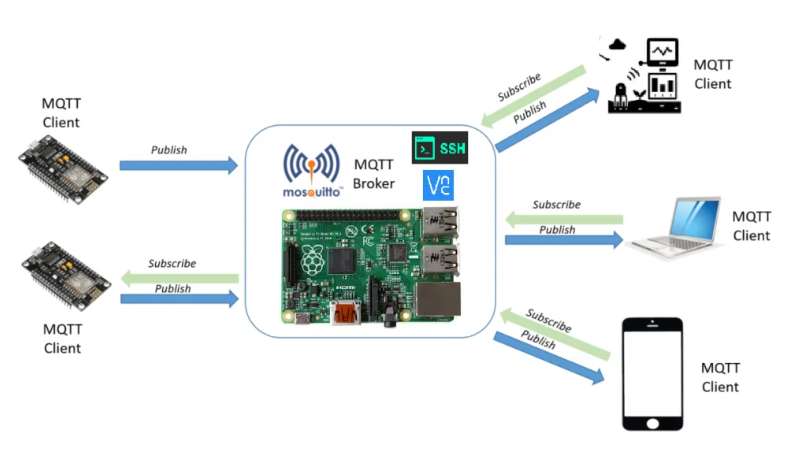
\includegraphics[width=150mm]{Imagem/CAP2/fluxo_mqtt.png}\\[0.10cm]
	Fonte: (Blog Eletrogate).
\end{figure}

%\begin{figure}[H]
%	\centering
%	\caption{Arquitetura de Aplicação do protocolo MQTT.}
%	\label{fig:fluxo_mqtt}   
%	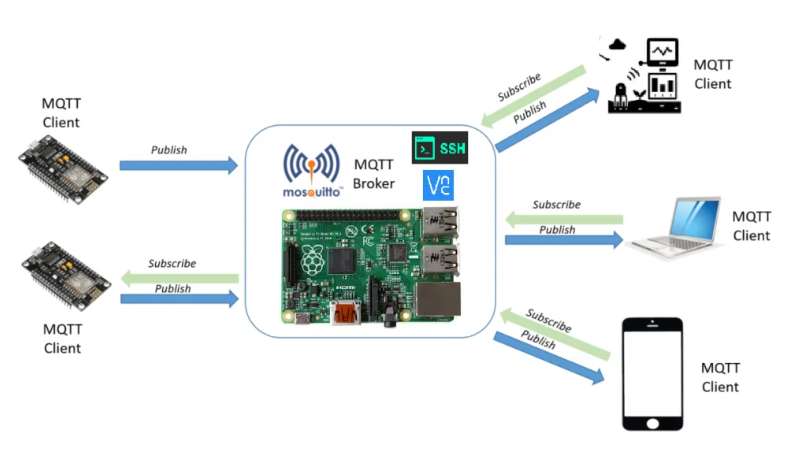
\includegraphics[width=150mm, height=100mm]{Imagem/CAP2/fluxo_mqtt.png}\\[0.10cm]
%	Fonte: (Blog Eletrogate).
%\end{figure}


\section{Linguagem \textit{Python}}

\textit{Python} é uma linguagem de programação interpretada de alto nível, destacada pela sua facilidade de aprendizado, sintaxe simples e compreensível e poder de integração com vários sistemas e softwares. Além disso, o Python possui uma abordagem poderosa de orientação objeto, o que aumenta a versatilidade das possibilidades de \textit{scripts} e aplicações da linguagem, sendo possível utilizá-la para automação residencial/industrial, desenvolvimento web, interfaces gráficas, manipulação de banco de dados, conexão e criação de arquitetura de redes como o MQTT, manipulação de arquivos de texto (TXT) ou dicionários (JSON), dentre outras \cite{python}. 

O interpretador Python e suas bibliotecas, são, em grande parte, gratuitas, leves e de fácil instalação, isso faz da linguagem amplamente utilizada em diversos âmbitos da tecnologia, dentre eles, os sistemas embarcados.

Na Raspberry Pi, o Python é a linguagem padrão e pre-instalada para controle de diversas ferramentas, como controle de \textit{GPIOS}, Automações e algumas configurações do sistema, a sua interface de programação (\textit{Integrated Development Environment - IDE}) padrão é o Thonny, que se destaca pela sua versatilidade e leveza para construção de programas em Python \cite{thonny}, uma vez que se encontra pré-instalado no \textit{RaspBian} \cite{Raspbian}. Para a instalação de bibliotecas diversas do python na Rasp, utiliza-se o comando ''\texttt{sudo pip3 install <Nome da Biblioteca>}'' no terminal de comando \cite{raspberrypi_foundation}, como visto na \autoref{fig:rasp_pi_install}.

\begin{figure}[H]
	\centering
	\caption{Raspberry Pi - Instalação de bibliotecas usando o \texttt{sudo pip3 install}.}
	\label{fig:rasp_pi_install}   
	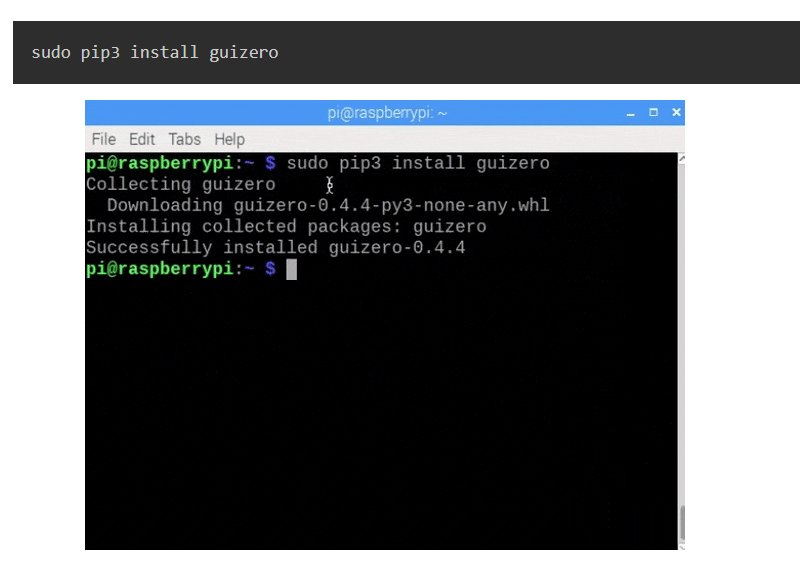
\includegraphics[width=100mm]{Imagem/CAP2/install_rasp.png}\\[0.10cm]
	Fonte: \cite{Pip_rasp}.
\end{figure}

\section{Reconhecimento Automático de Fala (Speech-to-Text - STT)}

O reconhecimento automático de fala, também conhecido como \textit{Speech-to-Text (STT)}, é uma tecnologia que permite converter sinais de áudio provenientes da fala humana em texto processável por sistemas computacionais. Essa tecnologia é amplamente utilizada em assistentes virtuais, sistemas de automação, interfaces homem-máquina e aplicações de acessibilidade.

O processo de reconhecimento de fala envolve a captura do sinal de áudio por meio de um microfone, seguido pelo processamento desse sinal para identificação de padrões linguísticos que correspondam a palavras ou frases da linguagem humana. Para isso, são utilizados modelos matemáticos e estatísticos treinados com grandes conjuntos de dados de fala, como cita Martin e Jurafsky \cite{jurafsky2023}.

Nos assistentes virtuais modernos, o reconhecimento de fala é responsável por transformar a entrada do usuário em texto, que posteriormente será interpretado por sistemas de processamento de linguagem natural ou modelos de linguagem (como os \textit{LLM's}), permitindo que o sistema execute comandos ou gere respostas adequadas.

\subsection{Biblioteca Vosk}

O \textit{Vosk} é uma biblioteca de reconhecimento de fala de código aberto baseada no \textit{framework Kaldi}, desenvolvida para aplicações offline e em dispositivos com recursos computacionais limitados, ou até mesmo sistemas como móveis como \textit{Android} e \textit{Ios}. A biblioteca oferece suporte para múltiplos idiomas e permite o reconhecimento de fala em tempo real, sendo compatível com diversas linguagens de programação, incluindo Python.

Uma das principais vantagens do Vosk é a capacidade de executar modelos de reconhecimento localmente, sem necessidade de conexão com servidores em nuvem. Essa característica é particularmente importante em aplicações que demandam maior privacidade de dados, baixa latência e funcionamento em ambientes sem acesso à internet.

Além disso, o Vosk apresenta boa compatibilidade com dispositivos embarcados, como a Raspberry Pi, possibilitando sua utilização em sistemas embarcados e projetos acadêmicos que envolvem interfaces de voz \cite{vosk}.

\section{Síntese de Fala (Text-to-Speech - TTS)}

O Text-to-Speech é uma tecnologia feita para converter através da síntese de voz entradas de texto em som, a interface é hoje utilizada por diversos fabricantes nos mais variados usos, como sistemas de acessibilidade, assistentes virtuais de voz e narração de livros. Os modelos de TTS utilizam aprendizado profundo (deep learning) para fazer uma Análise Linguística da entrada e então fazer a Síntese de voz utilizando codificação para converter texto em formas de ondas de som \cite{tts_ansi}.

No contexto das assistentes virtuais os sistemas TTS desempenham um papel importante na conversação, visto que gera uma resposta audível usuário que pode estar em outro cômodo, ou até mesmo ter necessidade deste tipo de recurso. A importância desse sistema é vista no trabalho feito por Rizqi Andry \cite{ardiansyah2016narrator}, onde o autor utiliza TTS para criação de um narrador eletrônico em um robô para pessoas cegas.

\subsection{A ferramenta eSpeak NG }
O \textit{eSpeak NG} é uma ferramenta de TTS compacta de código aberto e disponível para diversos sistemas operacionais, como \textit{Windows}, \textit{Linux} e \textit{Android}. Por ser compacto, o sintetizador possui baixo consumo de recursos computacionais, o que possibilita seu uso em computadores de placa única e sistemas embarcados como a Raspberry PI \cite{espeakng_git}. Além disso, o eSpeak possui ajuste de parâmetros como velocidade da fala, tonalidade e timbre da voz reproduzida, e suporte para diversos idiomas e variações linguísticas, incluindo o português.

Em seu uso, o eSpeak pode reproduzir textos no terminal de comando, utilizando seu executável, ou ser acessado como um sub processo do sistema operacional em uma linguagem de programação como o Python, onde é possível definir a velocidade com o parâmetro ''\textit{-s}'' e o tipo da voz (idioma e variação) com o parâmetro ''\textit{-v}''. A \autoref{fig:espeak} mostra um comando de utilização do eSpeak utilizando o parâmetro de velocidade em 160 (que representa 160 palavras por minuto (PPM)) e a variação linguística do português brasileiro ''\textit{mr-br3}'' para reprodução da mensagem ''Óla mundo!!''.

\begin{figure}[H]
	\centering
	\caption{Uso do eSpeak para TTS.}
	\label{fig:espeak}   
	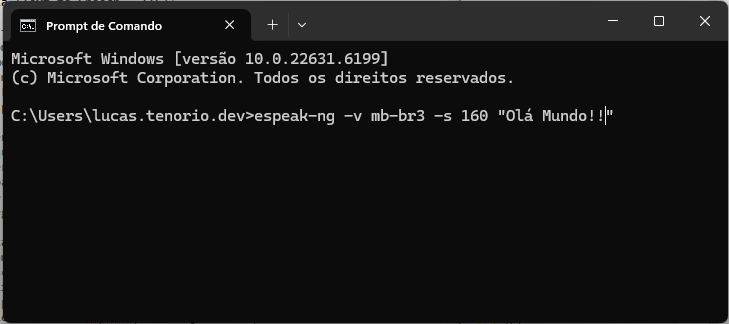
\includegraphics[width=100mm]{Imagem/CAP2/espeak.png}\\[0.10cm]
	Fonte: (Próprio autor, 2026).
\end{figure}


\section{Interface Gráfica do Usuário (\textit{GUI - Graphical User Interface})}
A Interface Gráfica do Utilizador, do inglês \textit{"GUI - Graphical User Interface"}, foi implementada pela primeira vez pela Xerox nos anos 70 e consiste em um modelo de interface para facilitar a interação do usuário de determinado sistema, permitindo a visualização, manipulação e configuração de forma visual e intuitiva. Este tipo de interface pode ser utilizada em diversos contextos, como automações industriais e residenciais, aplicativos de dispositivos móveis, \textit{Dashboards} de resultados e análise de dados.
No contexto de sistemas embarcados e aplicações de automação, interfaces gráficas desempenham um papel importante na visualização de dados, no gerenciamento de dispositivos e operação do sistema (como ativar  ou desativar Entradas e Saídas do hardware, configurar acesso a rede de comunicação, dentre outros), permitindo que o usuário acompanhe o funcionamento deste de forma clara e organizada. Dessa forma, a utilização de uma GUI contribui para melhorar a experiência do usuário e facilitar a interação com o sistema desenvolvido.
\subsection{A biblioteca PyQt}
O PyQt é uma biblioteca do Python para uso do QT, que é um framework criado em linguagem C++ multiplataforma projetado para criação de interfaces gráficas, ele possibilita aos desenvolvedores uma abordagem simples e acessível, além de possuir ferramentas de acessibilidade, acesso a banco de dados e compatibilidade com sistemas embarcados, como a Raspberry PI \cite{qt_site}. A companhia QT vende licenças comerciais, mas o QT é disponível em software livre para desenvolvimento de aplicações simples e	não monetizadas \cite{qt_about}.

\subsubsection{QT Designer}

O QT possui sua ferramenta gráfica, o QT Designer, que funciona como uma gerador  de códigos para manuseio dos Widgets ("Objetos" da tela) de forma visual, permitindo ao usuário montar sua aplicação e suas telas e visualiza-las antes mesmo de torná-la funcional, sendo uma interface poderosa de UX (User Experience) \cite{qt_about}. Como visto na \autoref{fig:QT_designer}, o QT Designer funciona como um sistema de criação de apps, ou seja, o usuário pode criar as telas com a resolução que preferir e escolher como irá configurá-la, a ferramenta possui uma vasta opção de elementos, como botões, entradas de texto, caixas de marcação, dentre outros, que são encapsulados em \textit{QWidgets} como forma de classes para uso em código Python.

\begin{figure}[H]
	\centering
	\caption{Ferramenta gráfica QT Designer.}
	\label{fig:QT_designer}   
	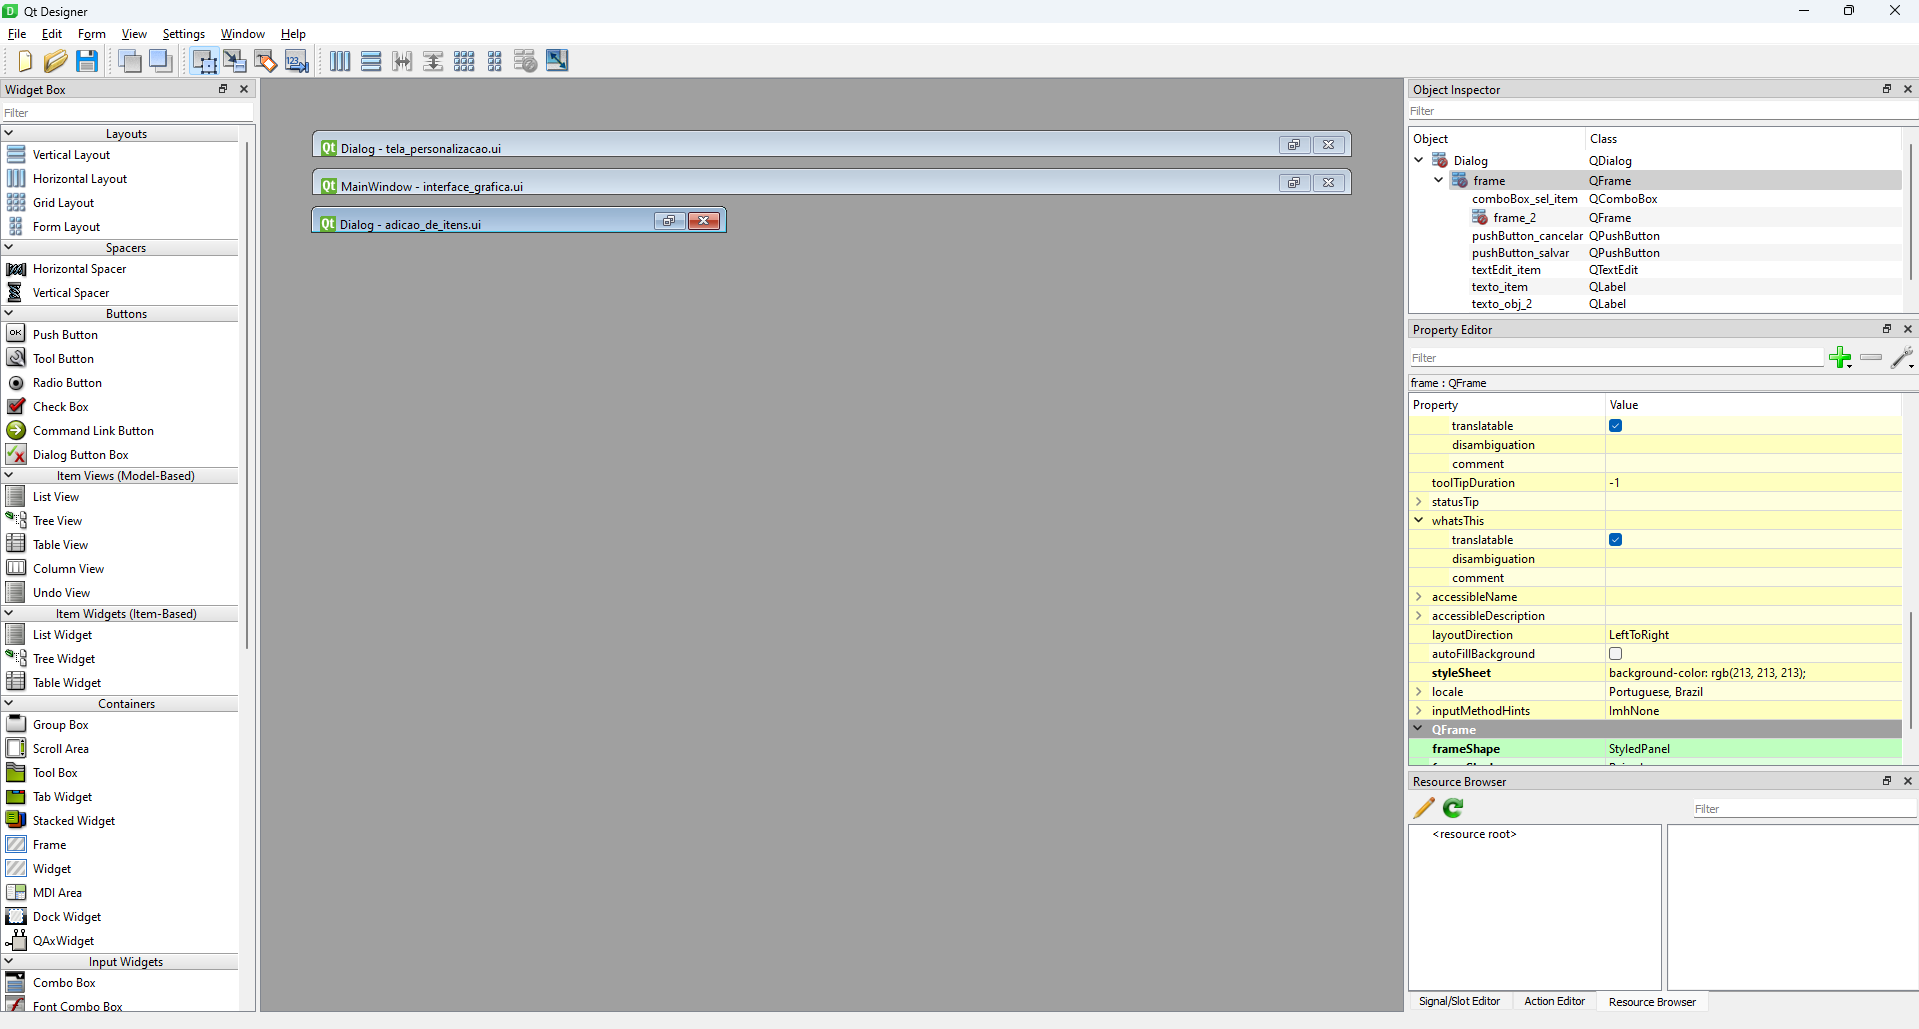
\includegraphics[width=0.9\textwidth]{Imagem/CAP2/QT_designer.png}\\[0.11cm]
	Fonte: (Próprio autor, 2026).
\end{figure}